%-----<<< BACKGROUND RESEARCH >>>-----
\chapter{Background}
\label{ch:background}

This Section provides background information related to our research. Basic concepts of FWMAV as well as the state-of-the-art research in the area is discussed in Section~\ref{sec:Flapping-wing vehicles}. Readers familiar with these concepts can skip the later sections, specifically Sections \ref{sec:cps}, \ref{sec:subsumption_arch}, \ref{sec:EA} and \ref{sec:MAS}.



\section{Related Research}
\label{sec:Flapping-wing vehicles}

Flapping-wing micro-aerial vehicles are relatively new research topic, with first concept papers appearing in early 2000's \cite{Shimada2000} \cite{Yan2001} \cite{Wood2001} \cite{Yan2001a}. To this date, the principles of flapping-wing flight are relatively well understood, including understanding of insect flight dynamics \cite{Stevenson1995} \cite{Fry2003} \cite{Dickinson1996} and related aerodynamics phenomena \cite{Birch2001} \cite{Sunada2001}. Researchers were able to successfully apply system identification methods (that were used on small-scale UAVs before, for example \cite{Hoffer2015}) on insects \cite{Taylor2003}, as well as on insect-size FWMAV \cite{Finio2011}. To this date, a free-flight of a fly-size FWMAV was achieved \cite{Chirarattananon} (although the power supply and data processing was external to the vehicle), as well as an untethered flight of a locust-size FWMAV with battery, sensors, radio and control unit on-board \cite{Rosen2016}. A comprehensive overview of modelling techniques is presented in \cite{Vm2015}.

First we will address the modelling and design of FWMAV, which is indeed very important for development of new vehicles and improvement of the existing prototypes. Then we will review several different approaches to the power system of a FWMAV, and discuss the commonalities and differences between them. Finally we will present most common on-board sensors that are a precursor of an autonomous FWMAV flight.

The most important part of the flapping-wing vehicle are the actuators (or "flight muscles"), since they provide propulsion to the robot. There are two main power technologies used -- either a brushed or brushless Direct-Current (DC) motor, or a piezoelectric oscillator. The DC motors are commonly used in larger robots and MAVs, but unfavourable scaling of magnetic forces limits the achievable power densities in small electromagnetic motors, making them unusable for the smallest fly-size FWMAVs \cite{Buck2013} \cite{Fuller2014}. Piezoelectric oscillators offer a better weight-to-light ratio, and be manufactured small enough for sub-centimetre robots. Yet they have a limited range of frequencies they can operate at, and require relatively high voltage of at least 150~Volts \cite{Wood2005} which makes them more difficult to work with. DC motors are more suitable for larger FWMAVs with take-off weight of a few grams. Piezoelectric oscillators are suitable for vehicles lighter than 1~gram. In both cases the actuators require a transmission, because neither DC motors, nor oscillators are suited to connect directly to the wings. 

\subsection{Oscillators}
\label{subsec:oscillators}

Piezoelectric bimorph oscillators consist of two layers of piezoelectric material, with another layer of flexible material in between as shown in Figure~\ref{fig:piezo}. When sufficiently high voltage is applied across the piezoelectric layers, one layer will expand while the other layer will shrink, causing a bending effect. Application of sinusoidal signal will result into oscillatory movement. Note that amplitude modulation of the driving signal changes minimal and maximal position of the oscillator, while applying an offset voltage shifts the middle position of the oscillator. Frequency modulation of the signal then changes the frequency of the oscillation \cite{Chirarattananon}. All three effects are important for control as will be shown later. Properties and design of piezoelectric bimorph oscillators were studied in great detail, we would refer the reader for example to \cite{Karpelson2012} and \cite{Wood2005}. An example of a FWMAV utilizing this type of actuator is shown in Figures~\ref{fig:robobee_example_1} and~\ref{fig:robobee_example_2}.

\begin{figure}
\centering
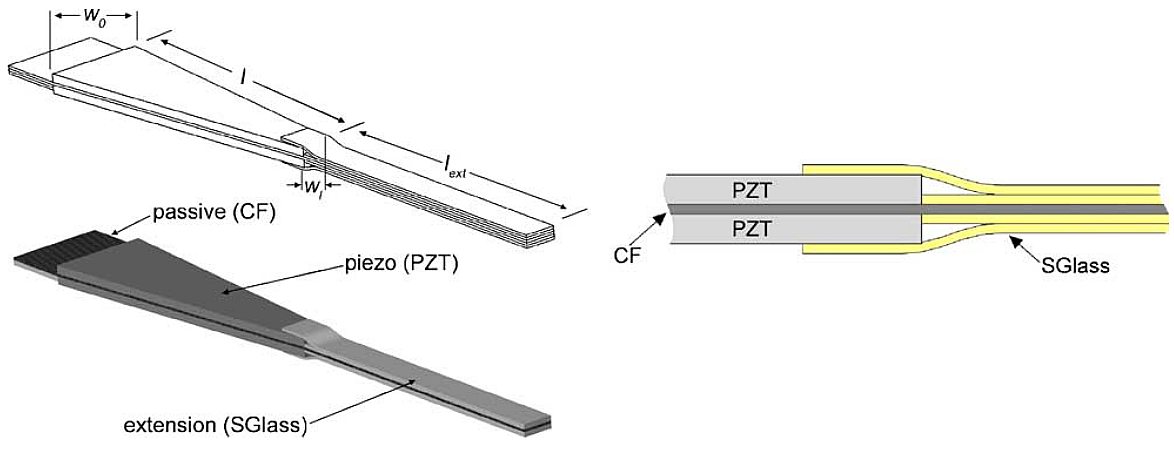
\includegraphics[width=0.8\textwidth]{Files/Figures/piezo.png}
\caption[Piezoelectric bimorph oscillator]{Piezoelectric bimorph oscillator \cite{Wood2005}. CF -Carbon Fiber, SGlass - a high stiffness fiberglass, PZT - Lead zirconate titanate}
\label{fig:piezo}
\end{figure}

% piezo oscilator example
\begin{figure}
\centering
\minipage{0.49\textwidth}
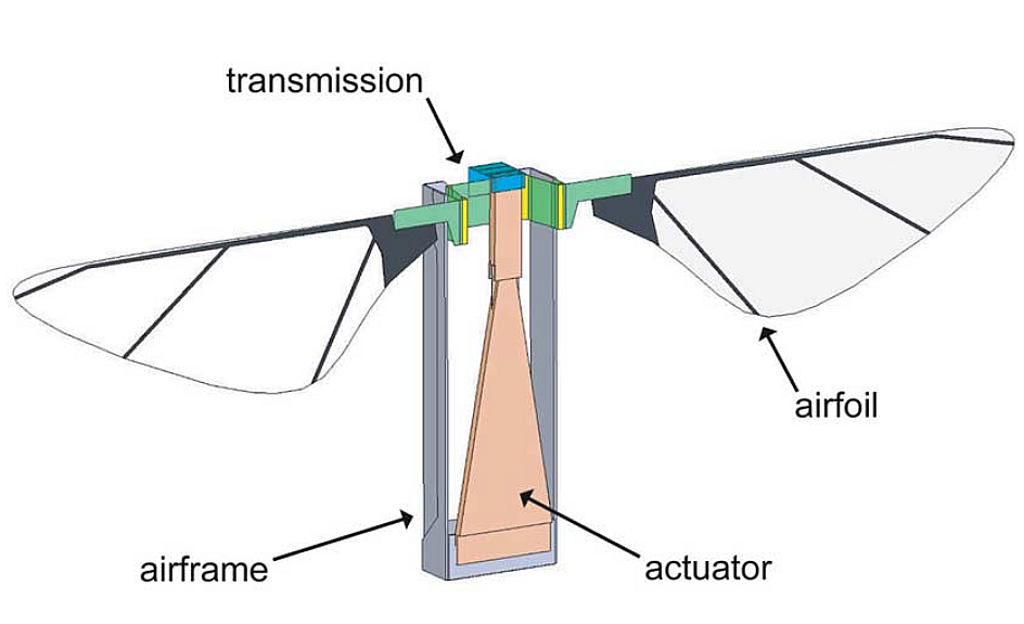
\includegraphics[width=\textwidth]{Files/Figures/robobee_example_1.png}
\caption[Piezo-oscillator conceptual drawing]{Conceptual drawing highlighting the main components of FWMAV utilizing piezoelectric oscillator \cite{Wood2005}}
\label{fig:robobee_example_1}
\endminipage\hfill
\minipage{0.49\textwidth}
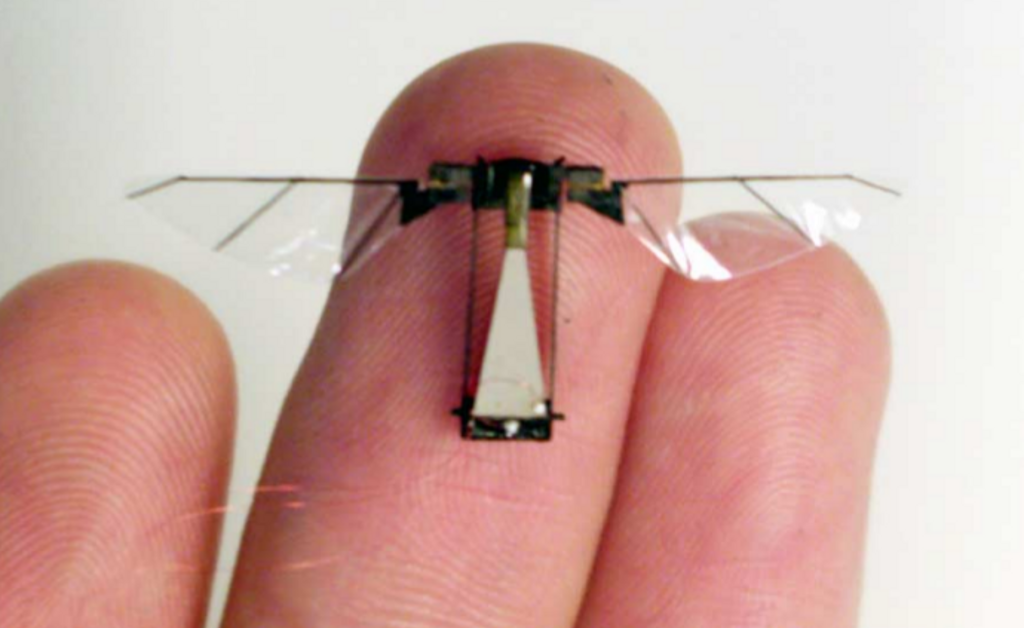
\includegraphics[width=\textwidth]{Files/Figures/robobee_example_2.png}
\caption[Piezo-oscillator in practice]{An assembled Robobee \cite{Wood2005}. Note the piezoelectric oscillator taking up most of the inner airframe.}
\label{fig:robobee_example_2}
\endminipage\hfill
\end{figure}

Flapping-wing flight is energetically costly \cite{Buck2013} as the inertia of the constantly oscillating wings has to be overcome in addition to the high aerodynamic drag \cite{Hines2015}, so it is essential to have as efficient power system as possible. One way, which was observed at fruit flies and blowflies, of achieving high efficiency and minimizing the additional inertia of the wings is to drive the wings at their mechanical resonant frequency, \cite{Hines2015}. Existing systems, such as \cite{Wood2008} were indeed designed to drive the wings at their resonant frequency.

The effect of resonant frequency is most obvious at the smallest scale (i.e. fly-scale robots), because the ratio of wings inertia to actuator inertia is large. A good example is a Harvard Robobee\cite{Wood2008} for which was this effect both theoretically predicted \cite{Yan2001} and experimentally measured (see in Figure~\ref{fig:resonance}). A linearized identified system model of the Robobee shows identical resonance frequency, as shown in Figure~\ref{fig:sysid}
As a result, a practical use of piezoelectric oscillators is challenging, because the oscillating frequency of the actuator has to match the resonance frequency of wings. Changing the oscillating frequency of the actuator is non trivial and depends on the size, shape, thickness and material of the oscillator \cite{Wood2005}. Oscillators also require a special driving circuitry with matched impedance for correct function \cite{Jafferis2016}. Finally the transmission is directly linked, so it changes torque ratios between the actuator and the wings, but can't change the frequency ratio (which is always 1:1).

\begin{figure}
\centering
\minipage{0.53\textwidth}
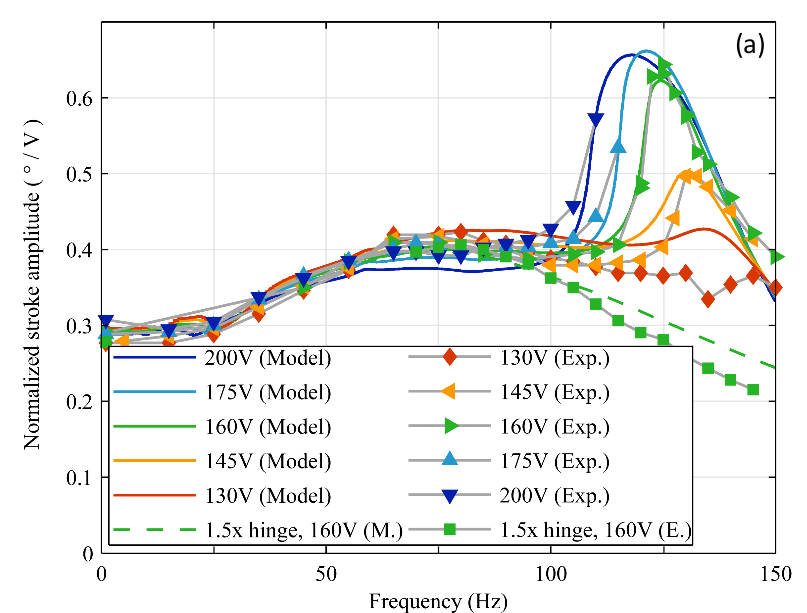
\includegraphics[width=\textwidth]{Files/Figures/resonance.png}
\caption[Resonance of the piezoelectric oscillator]{ Data and model fit for normalized stroke amplitude for various voltages applied to a piezoelectric oscillator. Note that for all applied voltages the resonance peak occurs between 110 and 130~Hz. Details of the experiment in \cite{Jafferis2016}}
\label{fig:resonance}
\endminipage\hfill
\minipage{0.45\textwidth}
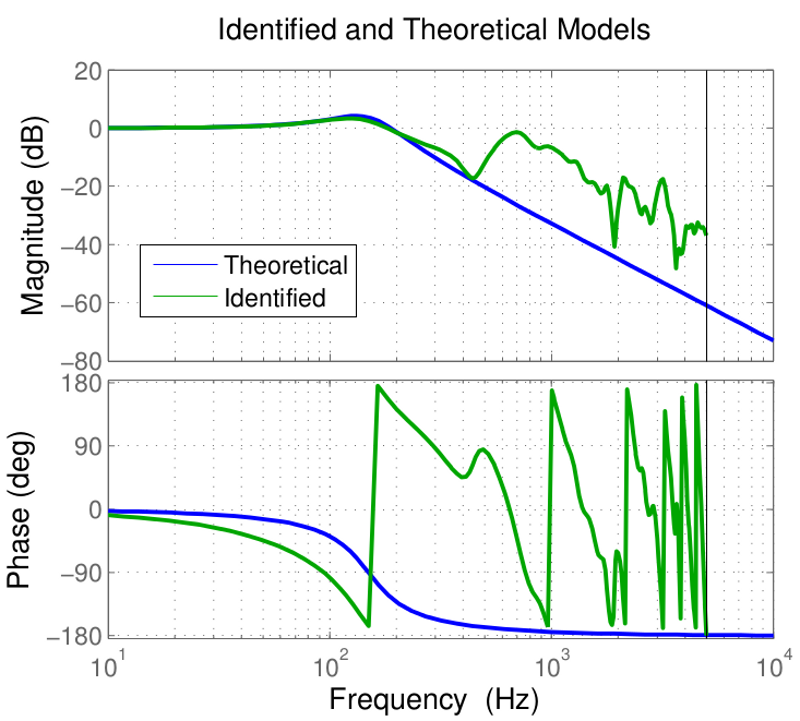
\includegraphics[width=\textwidth]{Files/Figures/sysid.png}
\caption[Bode plot of linearized Robobee model]{A bode plot of linearized theoretical model and identified model of Robobee \cite{Finio2011}. Note that in both models the resonance indeed occurs between 100 and 150~Hz which is consistent with observations.}
\label{fig:sysid}
\endminipage\hfill
\end{figure}


\subsection{DC Motors}
\label{subsec:dc_motors}
Using DC motors (both brushed and brushless) for wing actuation posses fewer challenges (in comparsion with the oscillators), at the cost of larger size and weight. They are also cheaper and easier to obtain, so as a result multiple FWMAVs with DC motors are available. The motor is connected to the wing via a transmission (typically with planetary gears) with various transmission ratio (from 25:1 to 4:1 depending on the size and type of the vehicle), as shown in Figure~\ref{fig:motor_and_wing}. Robots from different research groups differ mostly in how the wing is attached to the transmission, and whether additional gearing is used.

\begin{figure}
\centering
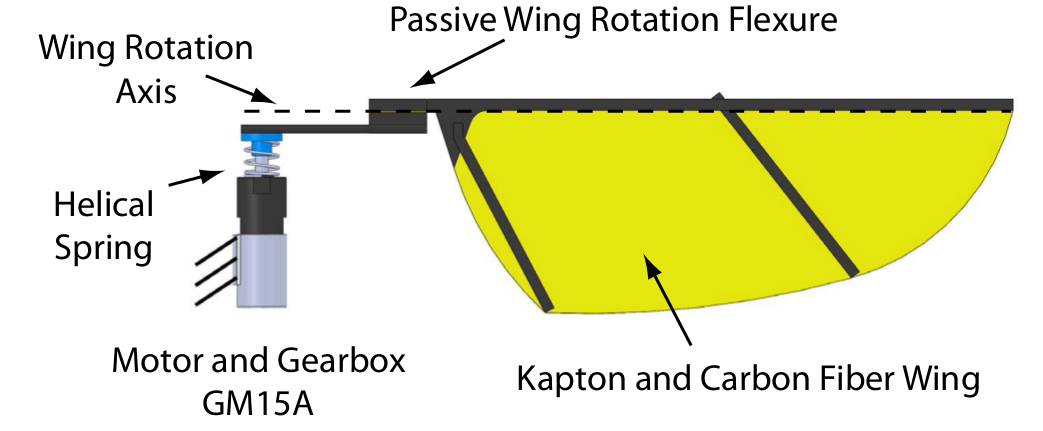
\includegraphics[width=0.8\textwidth]{Files/Figures/motor_and_wing.png}
\caption[DC motor and wing assembly]{An example of a motor driven wing: The motor drives the wing flapping angle through an attached gearbox. The wing passively rotates about a polyimide film and carbon fiber flexure. A spring is attached in parallel at the gearbox and wing spar connection. \cite{Hines2015}}
\label{fig:motor_and_wing}
\end{figure}

Probably the simplest approach is having a direct sliding crank going from the transmission and attached to both wings via flexible polyimide joints. That way only one actuator is required, but the control authority is limited and additional actuators are required for steering. This solution is also similar to the \textit{Dipteran} flight muscles of insects - an example is shown in Figures~\ref{fig:thorax} and~\ref{fig:simple_crank}. Needles to say, the mechanism shown in Figure~\ref{fig:simple_crank} doesn't produce enough lift for take-off and was built for demonstration purposes only.

% thorax + Dipteran-Insect-Inspired Thoracic gear
\begin{figure}
\centering
\minipage{0.49\textwidth}
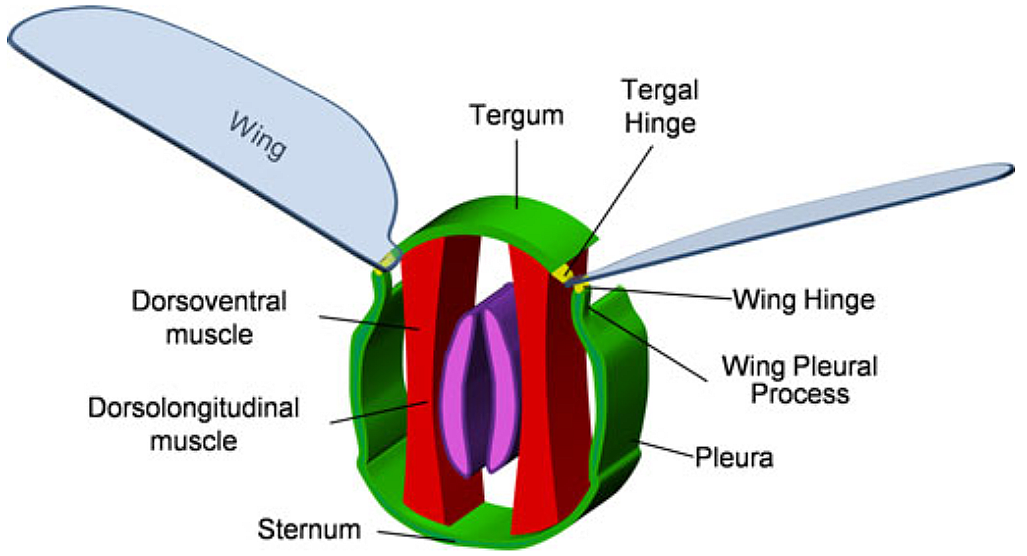
\includegraphics[width=\textwidth]{Files/Figures/thorax.png}
\caption[Dipteran insect’s flight thorax]{Dipteran insect’s flight thorax \cite{Lau2014} \newline \newline \newline}
\label{fig:thorax}
\endminipage\hfill
\minipage{0.49\textwidth}
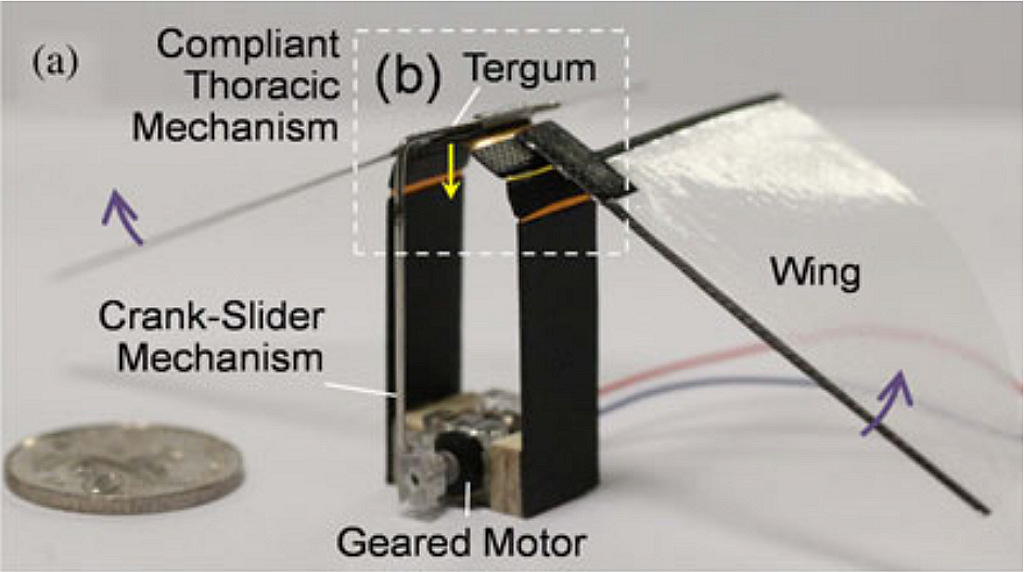
\includegraphics[width=\textwidth]{Files/Figures/simple_crank.png}
\caption[Simple crank mechanism]{Compliant thoracic mechanism with integrated polyimide film hinges for elastic energy storage. As the tergum of the thorax is depressed, its wings beat upwards \cite{Lau2014}}
\label{fig:simple_crank}
\endminipage\hfill
\end{figure}

More advanced version of the slider/crank mechanism also uses flexible polyimide joints, but is more compact as shown in Figure~\ref{fig:crank-slider}. This mechanism was developed for the previously mentioned 3.2~gram locust-size FWMAV (see Figure~\ref{fig:locust}) that is capable of free flights.

% second is the 3.2g platform (2016)
\begin{figure}
\centering
\minipage{0.49\textwidth}
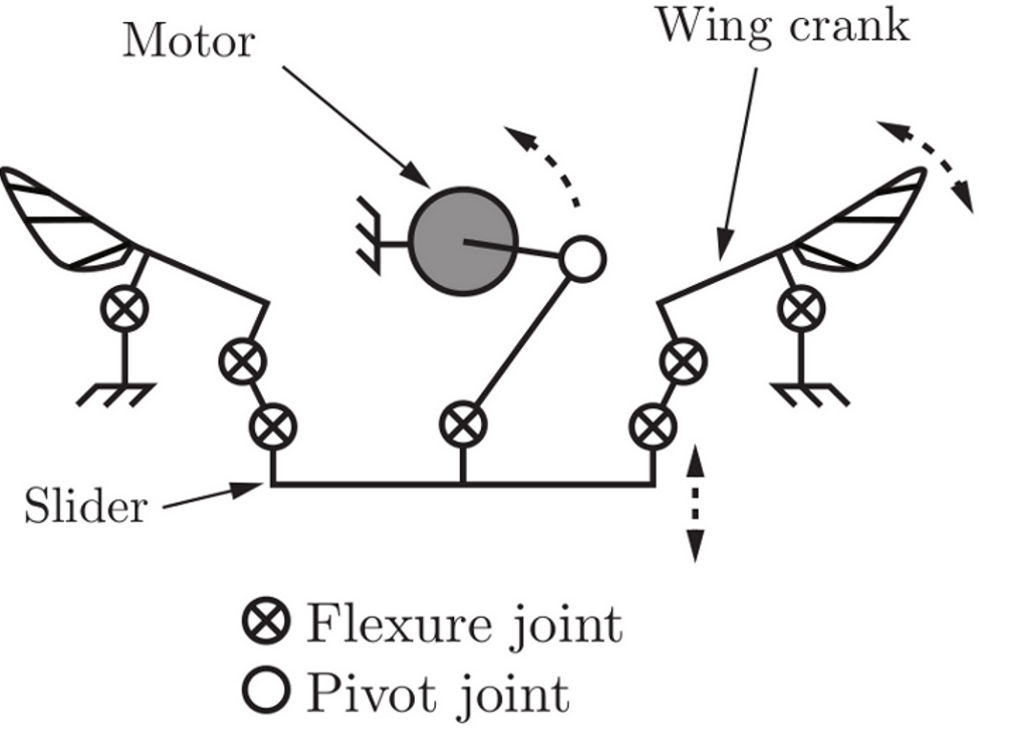
\includegraphics[width=\textwidth]{Files/Figures/crank-slider.png}
\caption[Crank-slider/slider-crank transmission]{Crank-slider/slider-crank transmission \cite{Rosen2016} }
\label{fig:crank-slider}
\endminipage\hfill
\minipage{0.49\textwidth}
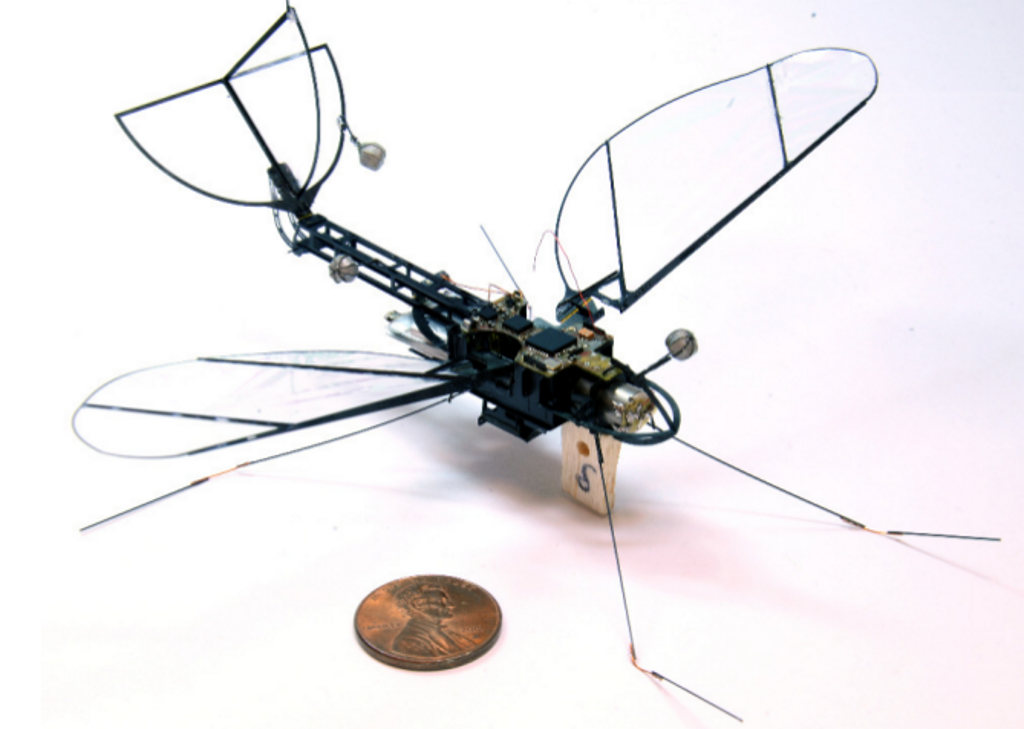
\includegraphics[width=\textwidth]{Files/Figures/locust.png}
\caption[Locust size FWMAV]{3.2~g untethered flapping-wing micro-air vehicle for flight energetics and control experiments \cite{Rosen2016}}
\label{fig:locust}
\endminipage\hfill
\end{figure}

Although planetary gears are prevalent for adjusting the motor output torque, some researchers employed multi stage gear reducer consisting of spur gears as the transmission \cite{Phan2015}. The advantage of this solution is a relative low-cost, since the gears can be 3D printed (unlike high-precision planetary gears), but the system is more susceptible to wear (since the gears are made form plastic) and is also more exposed to the environment. Figure~\ref{fig:gear_reducer} shows a detail of the gear reducer, and Figure~\ref{fig:gear_reducer_fwmav} shows the assembled FWMAV.

% third is Remotely Controlled flight of an Insect-like Tailless Flapping-wing Micro Ai (because they are using gears)
\begin{figure}
\centering
\minipage{0.49\textwidth}
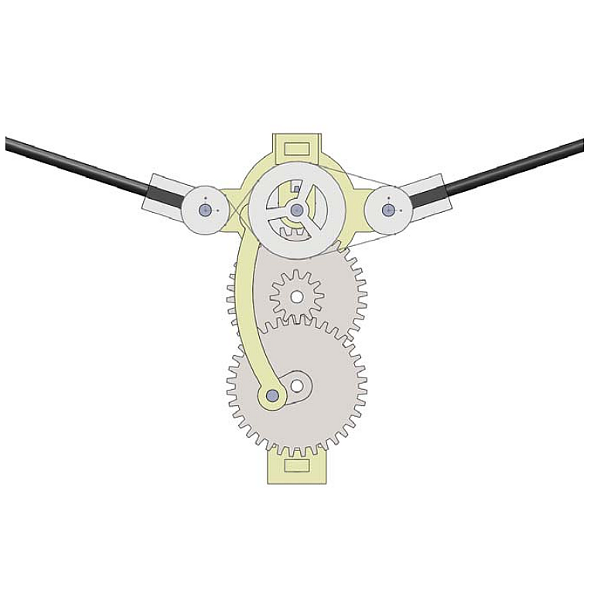
\includegraphics[width=\textwidth]{Files/Figures/gears.png}
\caption[Gear reducer with spur gears]{CAD model of the flapping-wing mechanism. \cite{Phan2015} Note the gear reducer, as well as additional linkages and levers.}
\label{fig:gear_reducer}
\endminipage\hfill
\minipage{0.49\textwidth}
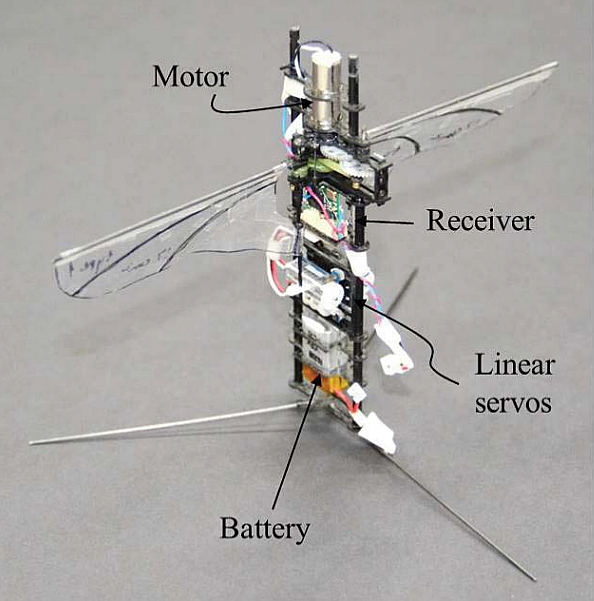
\includegraphics[width=\textwidth]{Files/Figures/gears_fwmav.png}
\caption[Assembled FWMAV with gear reducer]{Flapping-wing mechanism integrated control system and battery. \cite{Phan2015} This robot produces enough lift to carry its own weight.}
\label{fig:gear_reducer_fwmav}
\endminipage\hfill
\end{figure}

A system proposed by \cite{gallagher} utilizes a planetary gear transmission to match output torque of the DC motor (in this case a brushless), and rigid linkages to transfer rotary motion of the motor to wings. The advantage is that the system is more resilient than the one shown in Figure~\ref{fig:gear_reducer} (no need for small plastic gears), while still being relatively low-cost since all parts except the motor and the transmission are 3D printed. The CAD model of the assembly is shown in Figure~\ref{fig:our_wing_assembly_cad} while the whole assembly is shown in Figure~\ref{fig:our_wing_assembly_whole}.

% then we can show our robot (but will talk more about it later).
\begin{figure}
\centering
\minipage{0.49\textwidth}
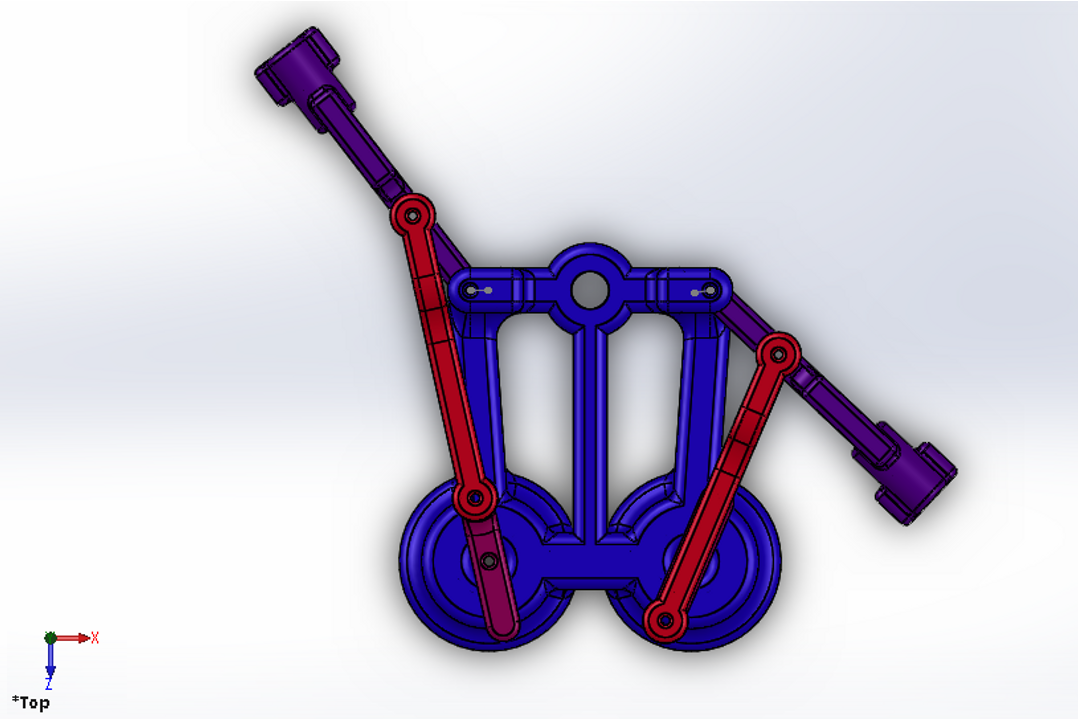
\includegraphics[width=\textwidth]{Files/Figures/cad_assembly.png}
\caption[Planetary gear transmission with solid linkages]{CAD model of the flapping wing mechanism \cite{cpsgroup}. Motors are connected to a planetary gear transmission (4:1 ratio), the output shaft of the transmission is then connected to rigid linkages that move the wings.}
\label{fig:our_wing_assembly_cad}
\endminipage\hfill
\minipage{0.49\textwidth}
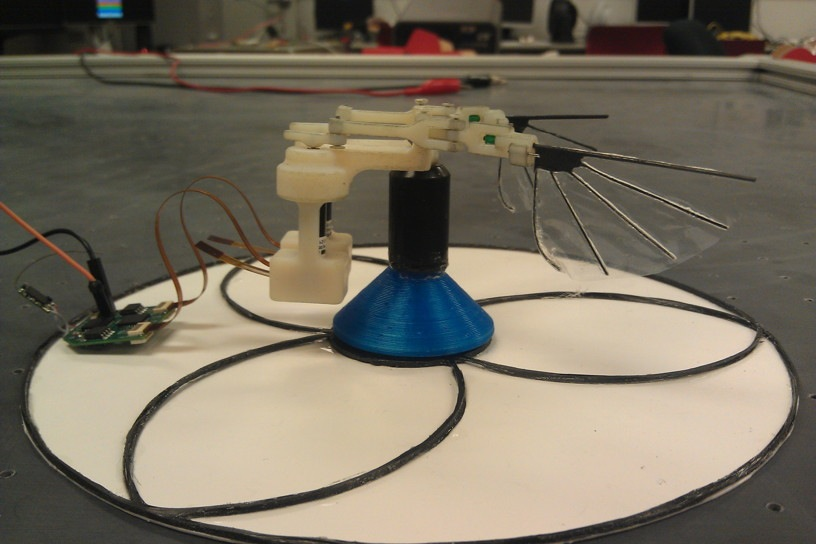
\includegraphics[width=\textwidth]{Files/Figures/sideview_vehicle_4x6.jpg}
\caption[Assembled FWMAV with planetary gear transmission]{Assembled flapping wing mechanism during tests. \cite{cpsgroup} \newline \newline \newline \newline}
\label{fig:our_wing_assembly_whole}
\endminipage\hfill
\end{figure}


% some conclusion - like hard to say what is better, depends on the application etc
As can be seen, a variety of FWMAVs exist, differing in the type of actuators (piezoelectric oscillators or DC motors) with different mechanical configuration. The multitude of designs suggests that different applications prefer unique configuration of FWMAV - depending on size, weight, required lift, price, manufacturability and maintainability, and many other factors. FWMAVs capable of free flight already exist, which is important because the results of our research can be used by other teams on their FWMAVs -- to add autonomy and fault recovery functionalities. In the next section we will review  on-board sensors available for FWMAVs.


\subsection{Sensors}
\label{sec:sensors}
The vast majority of experiments with FWMAVs is conducted indoors with the help of external vision system -- popular is for example a VICON vision system \cite{Wood2008} \cite{Rosen2016} \cite{Hines2015}. External vision sensors are great help during development and testing, but to make FWMAV truly autonomous onboard sensors are necessary, so the robots can explore and navigate in unknown environment. Since the application area expects operations in GPS-denied environments (such as inside buildings), GPS receivers cannot be used to determine position. GPS has also limited resolution (1-10~meters), which is insufficient However, sufficiently small and light GPS modules are already available, for example Telit SE880\cite{telit} weight only 80~mg (slightly more than the Hardvard Robobee) and is 4.7 x 4.7 x 1.4 mm (shown in Figure~\ref{fig:telit-se880}).

\subsection{Inertional Measurement Unit}
\label{subsec:imu}
% then sensors -> IMU etc (maybe from Rosen2016 - talk about gyros atd
Micro-Electro-Mechanical Systems (MEMS) gyroscopes and accelerometers are a good choice for FWMAVs. MEMS technology allows the sensors to be sufficiently small \cite{Rosen2016} - a good example is InvenSense MPU-9250 \cite{mpu9250} which combines 3-axis gyroscope, 3-axis accelerometer and 3-axis magnetometer in 3 x 3 x 1~mm package (see Figure~\ref{fig:mpu9250}). Together these sensors form an Inertial Measurement Unit (IMU) anbd their readings can be combined together to obtain attitude (and in some cases position) information. As the FWMAVs are improving their flight capability, the flight area they can cover is getting larger, which causes problems for the external camera systems that are dependent on conveniently placed markers - because the tracked robots are so small (compared to the area they flight in), the markers are also very small and are hard to distinguish in the camera (because of the finite camera resolution). Even in a very simple example of straight flight, raw gyroscope readings provided more insight into the FWMAV flight dynamics than the VICON system \cite{Rosen2016}.

% MPU size
\begin{figure}
\centering
\minipage{0.49\textwidth}
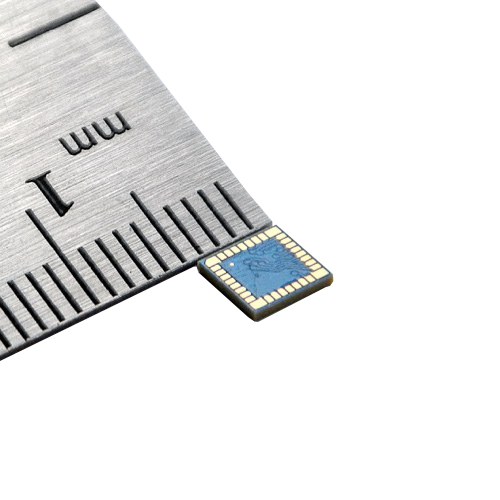
\includegraphics[width=\textwidth]{Files/Figures/se880.png}
\caption[Telit Jupiter SE880 GPS Module]{Telit Jupiter SE880 GPS Module \cite{telit}}
\label{fig:telit-se880}
\endminipage\hfill
\minipage{0.49\textwidth}
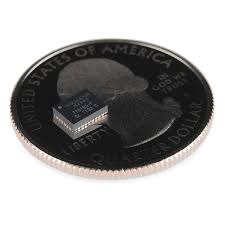
\includegraphics[width=\textwidth]{Files/Figures/mpu-9250.jpg}
\caption[InvenSense MPU-9259]{InvenSense MPU-9250 on a quarter dollar coin \cite{mpu9250}}
\label{fig:mpu9250}
\endminipage\hfill
\end{figure}

Gyroscopes measure rotational rates, and are reliable at higher frequencies, but suffer from a drift (a random walk caused by sensor noise). Accelerometers measure inertial acceleration, and work well at lower frequencies, but have bias that causes errors at higher frequencies \cite{Jensen2013}. Magnetometers measure the strength and direction of the local magnetic field. The magnetic field measured will be a combination of both the earth's magnetic field and any magnetic field created by nearby objects \cite{vectornav}. Magnetomers are used to improve heading (yaw) estimate.

Several sensor fusion algorithms are available. A simple, yet efficient, is a complementary filter - because gyroscopes and accelerometers are reliable at different frequencies, the complementary filter eliminates the unreliable frequencies for each sensor and then combines their output \cite{Jensen2013}. A Kalman filer (which is in fact an optimal linear estimator), an extended Kalman filter (which captures some nonlinear dynamics) and a particle filter, are popular algorithms of choice for sensor fusion \cite{simon_optimal_2006}. A good overview of available sensor fusion techniques is provided in \cite{Barton2012}.

\subsection{Vision Based Sensors}
\label{subsec:vision_based_sensors}
Although gyroscopes, accelerometers and even magnetometers have their equivalents in natural world, vision based navigation is perhaps the most familiar to us, because vision is our primary sense (as it is for many insects). The simplest approach is using optical flow for autonomous navigation, as was demonstrated on a 20-gram FWMAV with its own stereo vision system \cite{DeWagter2014}. Monocular optical flow was used for autonomous obstacle avoidance at high-velocities \cite{Barry2014}. Camera inputs can be not only used to navigate the FWMAV in an unknown environment, they can be also used to reconstruct a map of the environment in real time to create a model of the world around the FWMAV (in a process called Visual Simultaneous Localization And Mapping, or V-SLAM) \cite{Bibuli2007}, and to display the map to the operators so they have a better understanding of the explored area \cite{Bibuli2007a}. It was also demonstrated that a miniature optical sensor mimicking the function of ocelli (a type of a simple eye common to insects) can be carried onboard an FWMAV and used for stabilization and control \cite{Fuller2014}.

\section{Cyber Physical Systems}
\label{sec:cps}
The concepts presented here appeared in \cite{Greenwood2015}. Interested readers should consult that paper for more detailed information. We begin with the definition of an embedded system. Definitions vary, but essentially it is an information processing system where the end user is not aware a computer is
present. Examples include photocopiers, microwave ovens, engine control in automobiles and price scanners in markets and department stores. More formally, an embedded system is \textit{an information processing system embedded into an enclosing product.}

In general purpose computing performance, such as speed or virtually unlimited memory are major selling factors. Conversely, in embedded systems correctness is most important. Embedded systems often perform safety-critical operations where incorrect behavior can have dire consequences.

Embedded systems are ubiquitous. Applications include automobiles, commercial and military aircraft, weapon systems, medical equipment, smart power grids and transportation systems. They are becoming increasingly complex often including multiple processors, sophisticated communication networks and elaborate sensor and actuator systems. Sales of low-end microcontrollers suited for embedded applications exceed that of PC microprocessor sales and have done so for nearly 15 years.

So what exactly is a “cyber-physical system” (CPS)? Is it just another term for an embedded system? The short answer is no. The term CPS came into popular use as early as 2006 in large part via the efforts of Helen Gill at the U.S. National Science Foundation. A CPS is not a traditional embedded system or sensor net. The term CPS emphasizes the fact that computer resources (the cyber portion) are tightly integrated with a physical system (the physical portion). Cyber capabilities could be incorporated into every physical component. A CPS could have elaborate networks and may be reconfigurable. Control loops can be continuous or discrete. Cyber-physical systems exist at all scales from hand-held devices to power grids spanning large geographical areas. The commonly accepted definition of a CPS is as follows: \textit{A cyber-physical system is the integration of computation and physical processes.}

Figure~\ref{fig_cps} shows the abstract architecture of a CPS. Using the term "cyber-physical" emphasizes the strong link between the cyber and the physical worlds. In a CPS the cyber portion affects the physical system and the physical system affects the cyber portion. The integration of the cyber with the physical is extremely tight. In fact, this integration is so tight it may be impossible to identify whether the system behavior is due to computing or physical laws! For example, it may not be possible to tell if an unmanned aerial vehicle maneuver was caused by computer commands or resulted from the natural governing dynamics of the vehicle’s airframe. A CPS is not the union of the cyber with the physical but rather the intersection of the two.

FWMAV is a CPS because it contains both the \textit{cyber} portion - control loops, communication interface, path planning algorithms etc. as well as the \textit{physical} portion - motors to be rotated at a precise speed, wings to be controlled and flapped to produce light, and environment constraining the movement of the robot. 

\begin{figure}
\centering
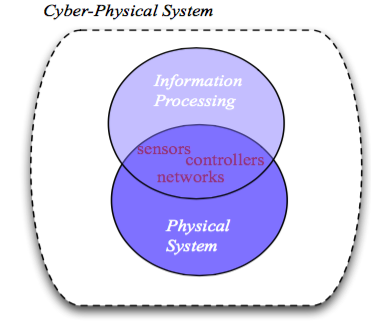
\includegraphics[width=0.5\textwidth]{Files/Figures/cps.png}
\caption[Cyber-Physical System]{An abstract view of the CPS architecture. The information processing system typically consists of one or more low-end microcontrollers. Sensors observe the physical system state while controllers provide inputs that alter the physical system state. Networks interconnect the physical and the cyber portions. The physical system can be electronic, mechanical or electromechanical.}
\label{fig_cps}
\end{figure}



% Then Subsumtion arch
\section{Subsumption Architecture}
\label{sec:subsumption_arch}
Readers familiar with the subsumption architecture may skip this section. A subsumption architecture\cite{brooks} is a very useful concept when we are dealing with:
\begin{itemize}
\item multiple goals
\item multiple sensor inputs
\item multiple actuators
\item requirements for robust and easily extensible solution
\end{itemize}

The subsumption architecture was first used to control an autonomous ground robot, capable of independent exploration and navigation in presence of obstacles in an office space. The main idea behind the subsumption architecture is to decompose the problem (i.e. navigation in presence of obstacles) into independent layers, and then assign priority to each of these layers. The layers are shown in Figure~\ref{fig_subsump}. The lower number, the higher priority of the layer. The benefit of the subsumption architecture is that it can model a complex behavior (such as trajectory following or navigation) by using simple rules that are easy to develop, modify and extend.

A \textit{dynamic subsumption architecture} is an extension of the concept, which allows the layers to be dynamically changed, more specifically: a change in the priority of the layers; add/remove layers; modify the consequents of the layers.

\begin{figure}
\centering
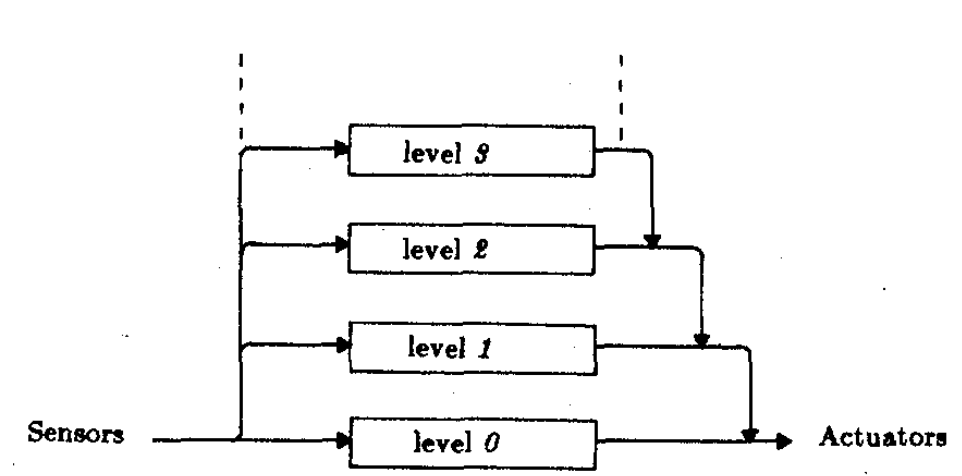
\includegraphics[width=0.8\textwidth]{Files/Figures/subsumption.png}
\caption[Subsumption architecture control layers]{Control is layered with higher level layers subsuming the roles of lower level layers when they wish to take control. \cite{brooks}}
\label{fig_subsump}
\end{figure}

Such change can be event triggered (e.g. a sudden change in the environment), or action triggered (i.e. the robot decides to change its behavior based on some internal state). Dynamic subsumption architecture allows the robot to react to changes in the environment (e.g. strong wind), in the robot itself (e.g. a damage to actuators, or low fuel), or in the mission (e.g. the mission was terminated by an operator); and its use for autonomous robots was already proven. 

Although the subsumption model was used for navigation and control of ground robots \cite{robot1, robot2}, it hasn't been used for flapping wing vehicles. Utilizing this powerful concept, we can easily develop and adapt the desired robot behavior. Note that the subsumption architecture was successfully applied in commercial products such as Roomba robot, scientific devices such as Sojuner Mars Rover and in military bomb disposal robots.


% Learning
\section{Evolutionary Algorithms}
\label{sec:EA}
In \textit{Evolutionary Algorithms} (EA) the new solutions to a problem are evolved from existing solutions by emulating Neo-Darwinistic evolution found in nature. Highly fit solutions -- i.e. those providing the best solution for the problem -- are preserved and further evolved, while solutions with low fitness are removed from the population. There are two types of evolution  relevant for CPS -- \textit{intrinsic} and \textit{extrinsic}~\cite{Greenwood2015}. The difference between \textit{intrinsic} and \textit{extrinsic} evolution is in how the fitness is determined. In \textit{extrinsic} evolution a computer model of the CPS is used, while in case of \textit{intrinsic} evolution the solution is downloaded to the CPS and physical tests are conducted. As a result, \textit{extrinsic} evolution is suitable for rapid evolution (because it can be run faster than real-time), but its accuracy depends on the model. \textit{Intrinsic} evolution on the other hand is more precise, but slower, because it has to be conducted on a physical device. 

An EA consists of a population of individuals, where each individual represents a particular solution to a given problem. New individuals are created from existing individuals via random mutation and recombination, but only the highly fit ones will survive. The fitness formula is dependent on the problem being solved. An EA runs for a fixed number of generations, at the end of the run the fittest individual is the final solution. The EA steps are shown in Algorithm~\ref{algo:ea}.
 
\begin{algorithm}
\caption{A basic evolutionary algorithm}
\label{algo:ea}
\begin{algorithmic}                    % enter the algorithmic environment
\STATE 1. Randomly generate the initial population;
\STATE 2. Evaluate the fitness of the initial population;
\WHILE{max number of generation not reached}
\STATE i. Select the best individuals for reproduction;
\STATE ii. Generate new individuals via random mutation and recombination;
\STATE iii. Evaluate the fitness of new individuals;
\STATE iv. Discard the least fit individuals;
\ENDWHILE
\end{algorithmic}
\end{algorithm}


To better show the idea, we present an example of a CPS with an EA: an evolvable hardware  -- a circuit that can be reconfigured to perform certain tasks, for example band pass filtering. In this case the fitness is determined by the filter performance (i.e. how precise is the band pass). The solution is encoded as a bitstring - representing configuration of the circuit. In case of \textit{extrinsic} evolution, a simulation is used to evaluate the fitness, while in case of \textit{intrinsic} evolution the response of the physical circuit is measured. Figure~\ref{fig:ea} shows the concept in detail.

\begin{figure}
\centering
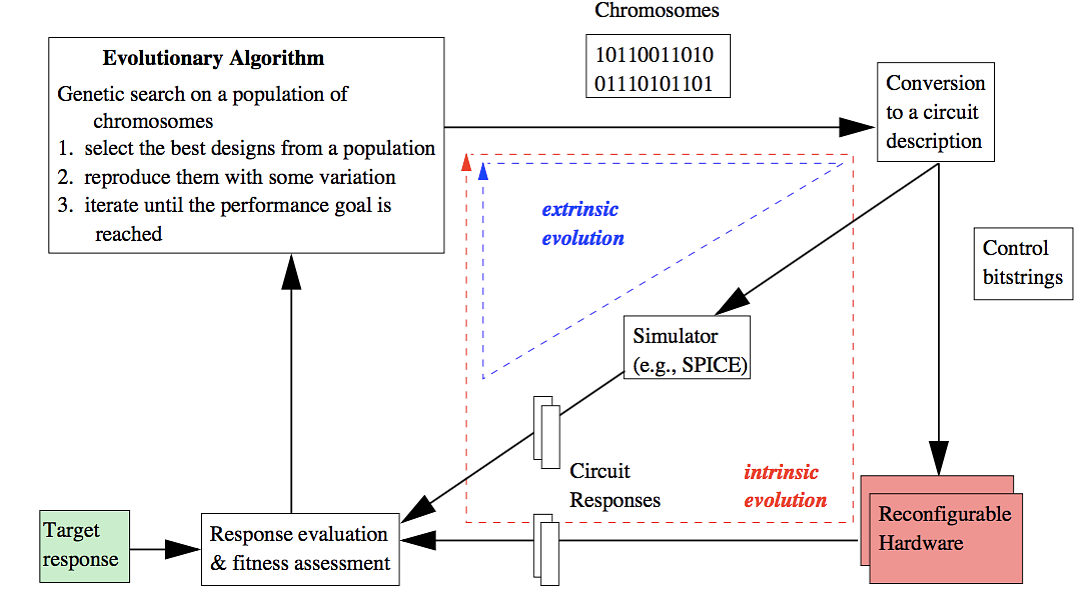
\includegraphics[width=\textwidth]{Files/Figures/EHW.png}
\caption[Evolutionary Algorithm]{Evolutionary Algorithm used in a CPS: evolving a bandpass filter on a reconfigurable hardware~\cite{Greenwood2015}.}
\label{fig:ea}
\end{figure}

% MAS
\section{Multi Agent Systems}
\label{sec:MAS}

To give the reader a better understanding of MAS, we define an agent as follows~\cite{Siekmann1814}:
\textit{An autonomous agent is a system situated within and a part of an environment that senses that environment and acts on it, over time, in pursuit of its own agenda and so as to effect what it senses in the future.} An agent receives \textit{percepts} from the environment, and generates \textit{actions} that might or might not depend on the \textit{percepts}. Figure~\ref{fig:agent} illustrates this idea. The agents can have different types, but for the purpose of our research we considered only \textit{Reactive agents}. These agents react to changes in the environment in a stimulus-response fashion by executing the simple routines corresponding to a specific sensor stimulation. A famous reactive agent architecture is the previously mentioned subsumption architecture~\cite{Siekmann1814}.

\begin{figure}
\centering
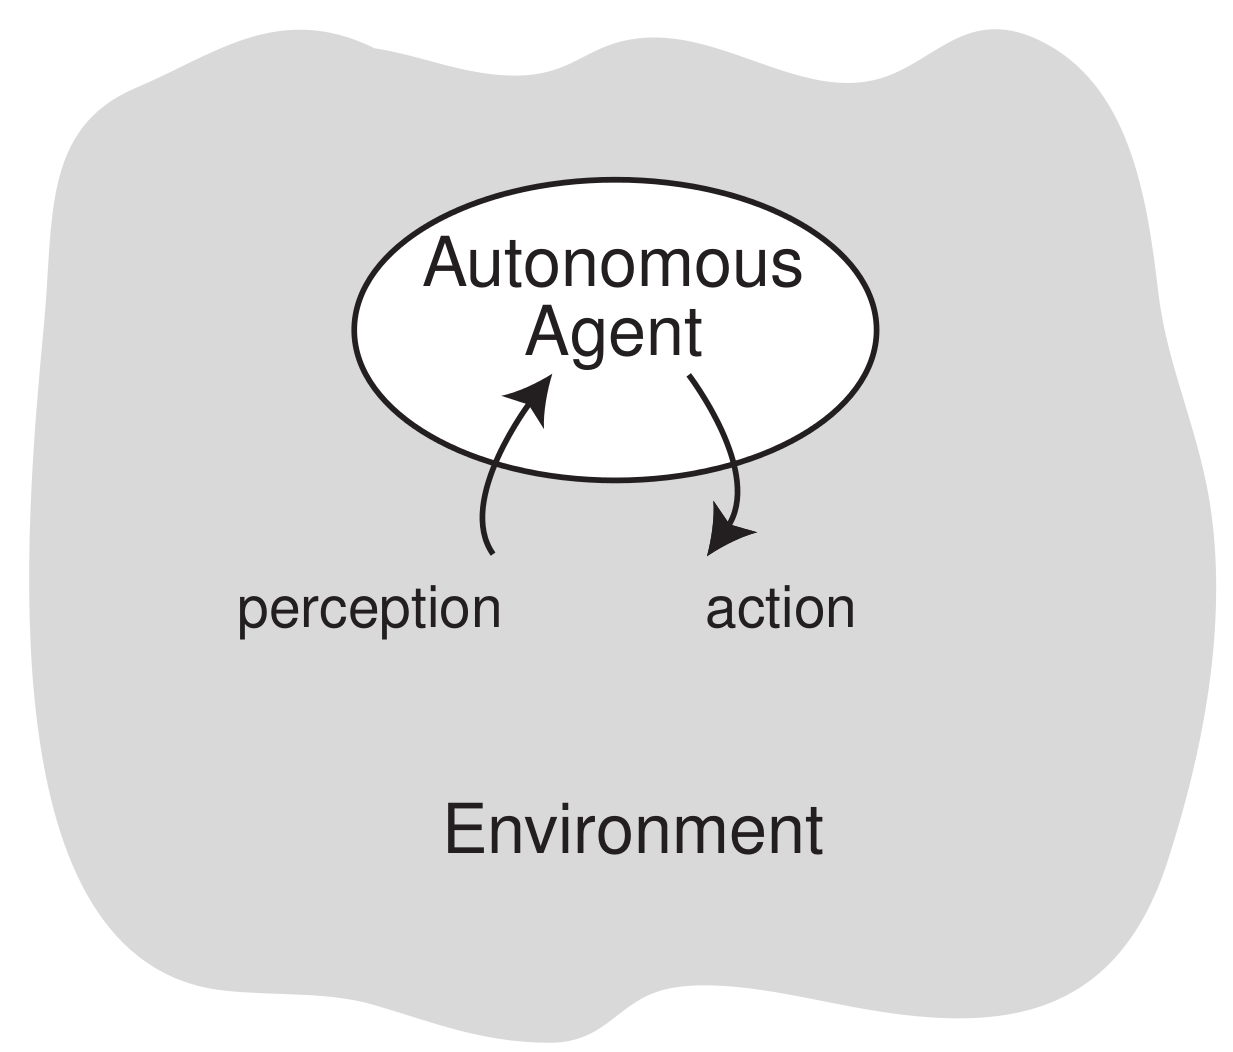
\includegraphics[width=0.6\textwidth]{Files/Figures/agent.png}
\caption[An autonomous agent and its environment]{An autonomous agent and its environment~\cite{Siekmann1814}.}
\label{fig:agent}
\end{figure}

Since multiple agents are used, they interact in some way. For our purposes we use \textit{cooperative} agents -- i.e. agents that work together to achieve some common goal (such as moving a robot to a certain place). Other interactions are also possible (some agents can be \textit{competitive} against each other), but not suitable for our research. The agents can communicate in multiple ways. The basic communication paradigms are these four~\cite{Siekmann1814} (Figure~\ref{fig:agent_com} illustrates the idea):
\begin{itemize}
\item \textit{Peer-to-peer} communication: messages are sent directly to specific agents. This is usually done by identifying the partners, for instance with an email-like address (message-passing-like communication). It is also possible that an intermediate channel takes charge of the transmission of the data, and that the partners of communication do not know each other.
\item \textit{Broadcast} communication: a message is sent to everybody in the MAS. Interested agents can evaluate the received data or ignore it.
\item \textit{Multicast} communication: A message is sent to a specific group of agents.
\item \textit{Generative} communication: communication is realized through a black-board: agents generate persistent objects (messages) on the black-board, which are read by other agents. The reading can be done independently of the time of the message generation; thus the communication is fully uncoupled.
\end{itemize}

\begin{figure}
\centering
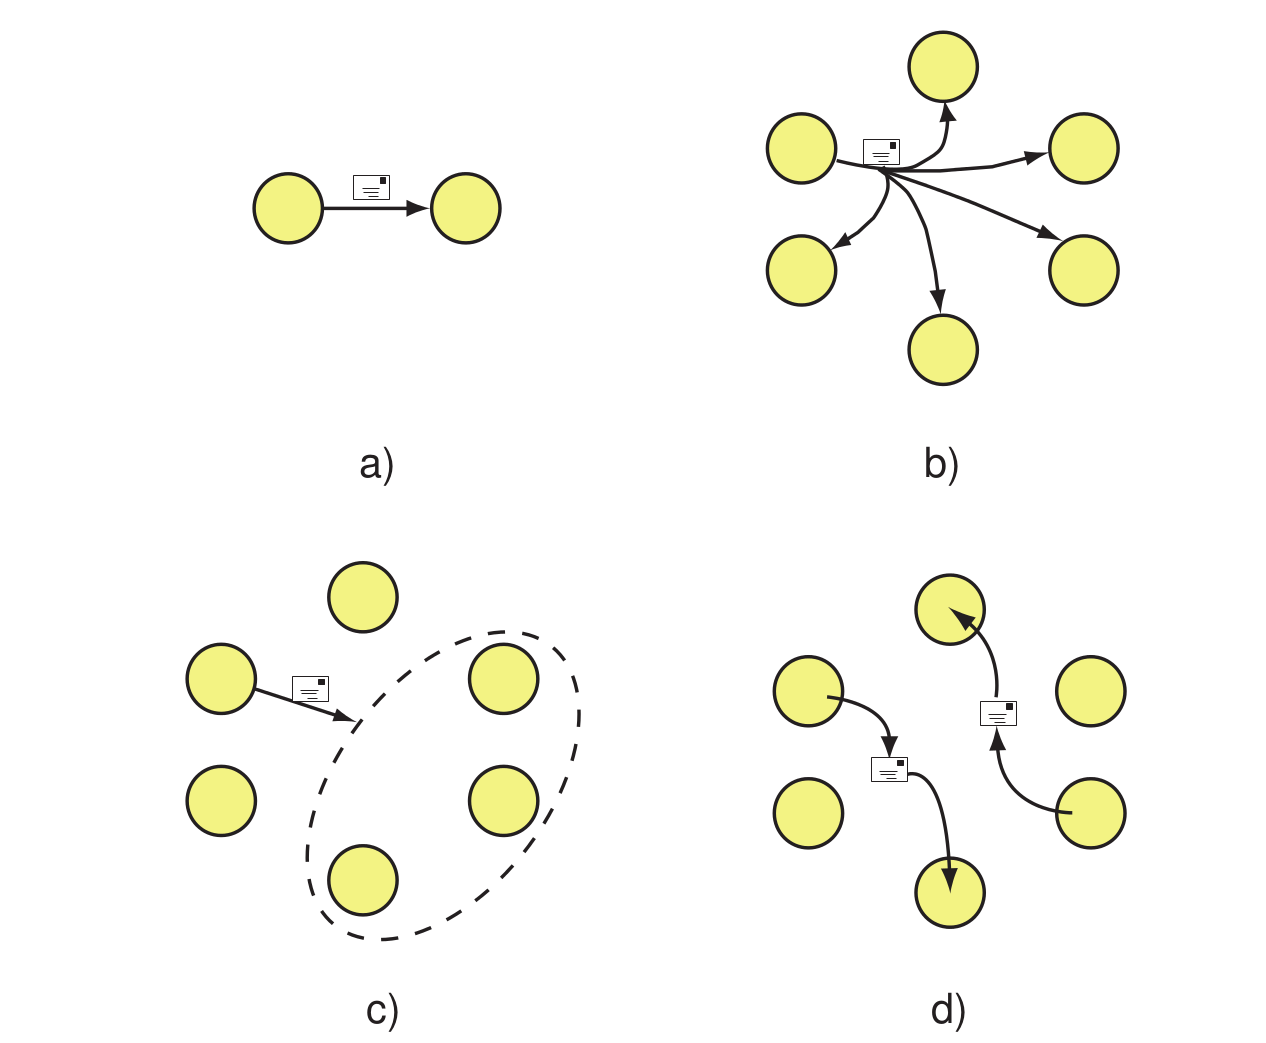
\includegraphics[width=0.8\textwidth]{Files/Figures/agent_com.png}
\caption[Basic communication paradigms]{Basic communication paradigms: a) peer-to-peer, b) broadcast, c) multi-cast and d) generative communication.~\cite{Siekmann1814}.}
\label{fig:agent_com}
\end{figure}

In summary, a MAS relies upon a number of agents (actors) that communicate with each other and typically cooperate in order to complete a certain task, such as target tracking \cite{Han2013} or mapping \cite{Kovacinal2002}. Although a MAS were successfully used for path planning of UAVs \cite{Shima2005} \cite{Chen2013}, convoy protection \cite{Ding2010} or flood monitoring \cite{Abdelkader2014}, it was never used for a control of a FWMAV.


This section showed the reader the bigger picture and research related to our work. In short, FWMAVs are more and more popular and there are many designs available, all utilizing two types of actuators - either a piezoelectric oscillator or a DC motor. Various modelling techniques exist, so it is possible to simulate the performance of a FWMAV before it is built, assuming we have enough information about individual subsystems. A multitude of sensors exist, as well as a wide range of sensor fusion algorithms for position and attitude estimation -- which can be applied on FWMAVs in a similar way as on larger UAVs (once sensors with sufficiently small footprints become available). A subsumption architecture has been used in robots before, achieving relative sophisticated intelligence with a simple set of rules. A MAS has never been used for a control of a FWMAV, although a MAS were also used in robotic applications. The next chapter formally defines the problem our research is solving, and provides details about the developed FWMAV and our experimental setup.
